\documentclass[12pt]{report}
\usepackage{listings}
\usepackage{amsthm}
\usepackage[utf8]{inputenc}
\usepackage[english]{babel}
\usepackage{tikz}
\usetikzlibrary{arrows}
\usepackage[T1]{fontenc}
\usepackage{float}
\usepackage{url}
\usepackage{geometry}
\usepackage{marginnote}
\usepackage{url}
\usepackage[autostyle]{csquotes}
\newtheorem*{definition}{Definition}
\theoremstyle{definition}
\newtheorem*{theorem}{Theorem}
\theoremstyle{theorem}
\lstdefinestyle{customc}{
	belowcaptionskip=1\baselineskip,
	breaklines=true,
	xleftmargin=\parindent,
    numbers=left,
    numberstyle=\ttfamily\color{gray},
	language=Java,
	showstringspaces=false,
	basicstyle=\footnotesize\ttfamily,
	keywordstyle=\bfseries\color{green!40!black},
	commentstyle=\itshape\color{purple!40!black},
	identifierstyle=\color{black},
	stringstyle=\color{orange},
}
\lstdefinestyle{customasm}{
	belowcaptionskip=1\baselineskip,
	frame=L,
	xleftmargin=\parindent,
	language=[x86masm]Assembler,
	basicstyle=\footnotesize\ttfamily,
	commentstyle=\itshape\color{purple!40!black},
}
\lstset{escapechar=@,style=customc}
\usepackage{caption}
\captionsetup{belowskip=15pt,aboveskip=4pt}

\begin{document}
\begin{titlepage}
	\centering
    \null
    \vfill
    {\Large\itshape Comparing Maintainability in Software Paradigms
    \par}
    \vspace{3.0cm}
	{\scshape 
    A thesis presented \par 
    by\par
	Marc Coquand\par
	to\par
    The Department of Computer Science\par
    \vspace{0.8cm}
	for a degree of\par
    Master of Science in Engineering\par
    in the subject of\par
    Interaction Technology and Design\par}
    \vfill
    Umeå University\par
    Supervised by Anders Broberg\par
	\today\par
\end{titlepage}
\clearpage
\thispagestyle{empty}

\clearpage\newpage
\thispagestyle{empty}

\begin{abstract} 

    This study's goal is to compare approaches to functional programs and
    object-oriented programs to find how it affects maintainability and code
    quality. By looking at 3 cases, we analyze, how does a functional approach
    to software architecture compare to an OOP (Object-oriented programming)
    approach when it comes to maintainability and code quality? TO BE REPLACED
    WITH CONCLUSION

\end{abstract}

\clearpage\newpage
\thispagestyle{empty}

\section*{Acknowledgements}

TODO

\clearpage\newpage
\thispagestyle{empty}

\tableofcontents
\newpage

% Introduction
\chapter{Introduction}\label{introduction}

Different schools of thoughts have different approaches when it comes to
building applications. There is one that is the traditional, object oriented,
procedural way of doing it. Then there is a contender, a functional approach, as
an alternative way to build applications. Functional programming originates from
1936 from Lambda calculus~\cite{Turner} and even though functional programming
is old, the industry most commonly use Object-oriented, imperative, languages
such as Java. (ADD\_REFERENCE usage statistics) As of today, defects in software
are still common place with the average defect rate being 15- 50 per 10000 lines
of code.~\cite{McConnell:2004:CCS:1096143} This indicates that the tools used
might be inefficient and improvements can be made. Also with defects being so
common engineers partly not only need new tools that decrease defects but also
need to ensure that for future developers the code is easy to modify so that
when defects show up they can easily be fixed. The software needs to be
maintainble to be of good quality.

Software quality can be divided into two different subparts: software functional
quality and software structural quality.~\cite{Pressman:2004:SEP:994110}
Software functional quality reflects how well our system conforms to given
functional requirements or specification and the degree of which we produce
correct software.  To check that the software is correct, software engineers
create tests. In order to create tests, the engineer employs various patterns
and tools in the code to make the code easier to test, such as Object-oriented
programming. They can also use static analysis and logical proofs to ensure
correctness. 

Software structural quality refers to how well the software adheres to
non-functional requirements such as robustness and
maintainability.~\cite{Pressman:2004:SEP:994110} Some of the maintainability
aspects, such as readability, is hard to measure quantitatively. By performing
semi-structured interviews, it is possible to investigate how well the code is
understood. 

In this thesis, the focus will be on Functional programming as a potential
solution to increase software quality. The aim is to investigate what makes
software maintainable and can those criterias that make software maintainable be
enforced and with Functional programming.Since functional programming is not the
most popular approach to software engineering today, it is worth taking into
consideration how employing functional programming might affect the readability
and maintainability of the software. If no one understands the code, how can
they maintain the software?  Since software engineering is so general the focus
will be specifically on servers. In servers, it is common to use a protocol
called REST to establish communication between servers and
clients.(ADD\_REFERENCE REST)  These servers are called RESTful APIs and will be
explained further in Chapter~\ref{background}.  As of today, it is up to the
developer to manually ensure that this protocol is followed. Nothing enforces
the developer to do it correctly unless the library implementation enforces it.
Popular frameworks, such as Express, however do not enforce this protocol.

This thesis will show that it is possible using Functional programming to
implement a server library that forces the user to make REST compliant servers.
By enforcing that compliancy, it would aid developers in improving the software
functional quality. By establishing the rules in Object-oriented programming
for maintainable software and translating those to functional programming and by
evaluating the readability of code written using the library, the study aims to
find how software structural quality is affected through the use of functional
programming.


% Theory 
\chapter{Theory}\label{theory} 

This chapter will cover how the system architectures are implemented in practice
for Object-oriented systems and functional systems to address the concerns
established in Chapter~\ref{background}. This chapter also aims to
introduce different ways we can compare these software paradigms on complexity,
both in testability and mental complexity. This way 

Exact definitions exist of OOP but not for Functional programming, however
both's stated goal is creating maintainable programs.  The way OOP aims to make
maintainable software is by emphasising encapsulation of state into
\textit{objects} and message passing. Functional programs emphasise moving state
to the edges of the program, making the core logic of the program pure and using
immutable data (defined in Section~\ref{functionalprogramming}). Data that is
immutable can not be changed after initialization. This is explained further in
Section~\ref{functionalprogramming} and Section~\ref{oop}. To prevent defects,
tests need to be written to check that the behavior works as expected, thus
testability is of concern when creating maintainable software.

While paradigms define how we build our applications, we still need design
patterns for structuring the source code. A design pattern is a template for the
developer when structuring their code to solve certain problems. For instance,
without design patterns, one could couple dependencies with logic which affects
maintainability. Coupling logic and dependencies causes problems later when
changing the dependency since that means that logic needs to be changed as well.
This study will present the patterns for OOP and functional programming in their
respective section. 

\section{Characteristics of Functional Programming}\label{functionalprogramming}

 While different definitions exist of what Functional programming means, we
 define functional programming as a paradigm that uses of pure functions,
 decoupling state from logic, using trait-based polymorphism and
 immutable data.

\begin{description}
\item[ Purity ]

When a function is pure it means that calling a function with the same arguments
        will always return the same value and that it does not mutate any value.
        For example, given $f(x) = 2\cdot x$, then $f(2)$ will always
        return $4$. It follows then that an impure functions is either dependant
        on some state or mutates state in some way. For example, given $g(x) =
        currenttime \cdot x$, $g(5)$ will yield a different value depending on
        what time it is called. This makes it dependant on some state of the
        world. Or given $x=0$, $h()=x+1$. Then $h()$ will yield $x=1$ and $(h
        \circ h)()$ will yield $x=2$, making it impure.~\cite{wikipedia_pure}

	\item[ Trait-based polymorphism ]

		OOP inherits classes that contain methods and
attributes.~\cite{Gamma:1995:DPE:186897} Functional programs instead
define classes that describe the actions that are possible. For example, a
class \texttt{Equality} could contain a function \texttt{isEqual} that checks
if two data types are equal. Then any data type that implements the interface
Equality, for example lists or binary trees, would be able to use the function
isEqual.  This is known as type-classes in
Haskell\footnote{\url{www.learnyouahaskell.com/types-and-typeclasses}}, mixins
in Javascript\footnote{\url{www.typescriptlang.org/docs/handbook/mixins.html}}
or traits in Scala\footnote{\url{https://docs.scala-lang.org/tour/traits.html}}.

\item[ Immutable data by deafult ]

Immutable data is data that after initialization can not change. This means if
we initialize a record, \texttt{abc = \{a: 1, b: 2, c: 3\}} then \texttt{abc.a
= 4} is an illegal operation. Immutable data, along with purity, ensures that
no data can be mutated unless it is specifically created as mutable data.

\item[Decoupling state from logic]

Even if functional programs emphasise purity applications still need to deal
        with state somehow. For example a server would need to interact with a
        database. Functional programs solve this by separating pure functions
        and effectful functions. Effects are observable interactions with the
        environment, such as database access or printing a message.  While
        various strategies exist, like Functional Reactive
        Programming\footnote{Read more:
        \url{en.wikipedia.org/wiki/Functional_reactive_programming}},
        Dialogs\footnote{Read more:
        \url{stackoverflow.com/questions/17002119/haskell-pre-monadic-i-o}} or
        uniqueness types\footnote{Read more:
        \url{https://en.wikipedia.org/wiki/Clean_(programming_language)}}, the
        one used in Haskell (the language used in this thesis to construct the
        programs) is the IO monad. For the uninitiated, one can think of Monads
        as a way to note which functions are pure and which are effectful and
        managing the way they intermingle. It enables handling errors
        and state.\footnote{This is simplified as Monads are notoriously
        difficult to explain.}. 

As a strategy to further separate state and logic, one can construct a
        three-layered architecture, called the three layer Haskell cake. Here,
        the strategy is that one implements simple effectful functions,
        containing no logic as a base layer. Then on a second layer one
        implements an interface that implements a pure solution and one
        effectful solution. Then on the third layer one implements the logic of
        the program in pure code. The way the second layer is implemented is
        explained further in Section~\ref{interpreterpattern}. 
\end{description}

So while no exact definition of Functional programming exist, this thesis
defines it as making functions pure and inheritance being based around
functionality rather than attributes.

\subsection{ADTs: Sum types and product types}\label{types}

A type is in Haskell a \textit{set} of possible values that a given data can
have. This can be $int$, $char$ and custom defined types. A \textit{sum type} or
\textit{union type} is a type which is the sum of types, meaning that it can be
one of those it's given types. For example the type \texttt{type IntChar = Int |
Char} is either an Int or a Char. A useful application for sum types are enums
such as \texttt{type Color = Red | Green | Blue}, meaning that a value of type
Color is either red, green or blue. A sum type can be used to model data which
may or may not have a value, by introducing the Maybe type: \texttt{type Maybe
value = Just value | Nothing}.A product type is a type which is the product of
types, for example \texttt{type User = User Name Email}.  Informally, a product
type can be likened to a record in Javascript.  This allows us to model
computations that might fail. For example given $sqrt(x) = \sqrt{x},\, x\in
\mathbb{Z}$ then $sqrt(-1)$ is undefined and would cause Haskell to crash.
Instead by introducing a function \texttt{safeSqrt}, where \texttt{safeSqrt x =
if x > 0 then Just (sqrt x) else Nothing}, the program can force the developer to
handle the special case of negative numbers. Sum types are useful for
implementing the Interpreter pattern, explained in
Section~\ref{interpreterpattern}.

\subsection{GADT}\label{gadt}

a GADT is a \textit{generalized abstract data type}.  They specify, depending on
the input, what the output should be of that type. GADT enables implementing
\textit{domain-specific languages} (DSL). A DSL is a language with a limited
scope for specific applications. For example a parsing library or a calculator.

\begin{figure}[H]
    \begin{lstlisting}
        data Calculator = Number Int         
          | Add Calculator Calculator 
          | Multiply Calculator Calculator 
    \end{lstlisting}
    \caption{A Calculator GADT with two operations add and multiply.}
    \label{gadtcalculator}
\end{figure}

\begin{figure}[H]
    \begin{lstlisting}
        mathExpression = (Number 5 `Add` Number 3) `Multiply` (Number 4 `Add` Number 3)
    \end{lstlisting}
    \caption{A mathematical expression constructed using the GADT in
    figure~\ref{gadtcalculator}}
    \label{mathexpressiongadt}
\end{figure}


Figure~\ref{gadtcalculator} defines a GADT for a calculator. The calculator can
do two operations, add and multiply. This allows us to construct mathematical
expressions. The expression in Figure~\ref{mathexpressiongadt} can translates to
$(5+3)*(4+3)$ by defining a way to evaluate the expression.
Figure~\ref{calculator} defines an evaluation for the program.

\begin{figure}[H]
    \begin{lstlisting}
        evaluate :: Calculator -> Int
        evaluate (Add expr1 expr2) = evaluate expr1 + evaluate expr2
        evaluate (Multiply expr1 expr2) = evaluate expr1 + evaluate expr2
    \end{lstlisting}
    \caption{Evaluator for the calculator}
    \label{calculator}
\end{figure}

\subsection{Type classes}\label{typeclass}

A type class is a construct that allows for ad hoc polymorphism. This allows to
create constraints to type variables in parametrically polymorphic types. In
English, that means that it allows creating interfaces that must be implemented
for the types. For example the equality type class, defined in
Figure~\ref{equalitytypeclass}

\begin{figure}[H]
    \begin{lstlisting}
        class Eq a where
          (==) :: a -> a -> Bool
          (/=) :: a -> a -> Bool
    \end{lstlisting}
    \caption{Equality type class in Haskell.}
    \label{equalitytypeclass}
\end{figure}

By defining an Equality type class one can create general functions that can be
used for anything that is ``equalable''. For example Figure~\ref{printifequal}
is a function that prints a text if two items are equal. This function can be
used for floats, ints, tuples and everything else that implements the
\texttt{Eq} type class. Other uses for type classes is Num which implements
numeric operations for floats and integers. This is useful for implementing the
MTL technique which will allow us to implement the Interpreter pattern which
will be described in the following sections.

\begin{figure}[H]
    \begin{lstlisting}
        printIfEqual :: Eq a => a -> a -> IO ()
        printIfEqual a b =
            if a == b then
                putStrLn "They are equal"
            else
                putStrLn "They are not equal"
    \end{lstlisting}
    \caption{A function that prints a text if the two items are equal.}
    \label{printifequal}
\end{figure}


\subsection{Brief introduction to Monads for side effects}\label{monads}

Monads\footnote{\url{en.wikipedia.org/wiki/Monad_(functional_programming)}} are
a way to sequence computations that might fail while automating away boilerplate
code. Figure~\ref{monadclass} shows how Monads are implemented as a typeclass in
Haskell. It implements the function \texttt{return}, the function bind
\texttt{(>>=)}, the function sequence \texttt{(>>)} which is bind whilst
ignoring the prior argument and \texttt{fail} which handles crashes.

\begin{figure}[H]
    \begin{lstlisting}
        class Monad m where  
            return :: a -> m a  
            (>>=) :: m a -> (a -> m b) -> m b  
            (>>) :: m a -> m b -> m b  
            fail :: String -> m a  
            fail msg = error msg 
    \end{lstlisting}
    \caption{Monad type class in Haskell.}
    \label{monadclass}
\end{figure}

Informally, Monads are as a design pattern that allows us to sequence different
computations. Without them the developer would have to explicitly check if a
computation has failed. For example, given the function $unsafeSqrtLog =
sqrt\,\circ\,log$, then $unsafeSqrtLog(-1)$ would throw an error since $log$ and
$sqrt$ are undefined for $-1$.  Section~\ref{types} showed how the \texttt{Maybe
value} type could be used to create a safe computation \texttt{safeSqrt}.  To
sequence that computation with a function \texttt{safeLog}, the user would have
to manually check that \texttt{safeSqrt} returned a value \texttt{Just result}
and not \texttt{Nothing}. Monads allows sequencing these computations without
explicitly writing this check, so composing \texttt{safeSqrt} and
\texttt{safeLog} using bind becomes \texttt{safeSqrtLog n = safeSqrt n >>=
safeLog}. The same idea applies for effectful computations such as fetching data
from a database.

\subsection{Interpreter pattern for testability}\label{interpreterpattern}

The beginning of this chapter briefly mentioned that design patterns are
important to create maintainable software.  In this study a design pattern
called the Interpreter pattern will be used to structure functional programs. An
interpreter is something which interprets input of some format, modifies it and
transforms it into some output.  Informally, the interpreter pattern is a way to
create smaller composable compilers that when added together make one big
application. A compiler is a program that takes some input, interprets the input
and then does some output. A server, for example, would take some request,
interpret that request and then turn it into a response. The server could
integrate itself with the database, which would take some query, interpret that
query and then return an object.~\cite{interpreterpattern}

To implement this pattern in Haskell, create an Abstract Syntax Tree (AST) using
a sum type, of the program that contains all the available commands that the
program is capable of doing. See Figure~\ref{freeunion} for an example of a
to-do list AST. Once we have the AST we can encode the logic of the program as
instructions. Then the final step is to implement an interpreter for the program
that evaluates those commands. So if we have the commands in
Figure~\ref{freeunion}, we implement a function \texttt{eval} that takes a
command and computes some effectful code.  The command \texttt{Add Item (Item ->
next)} could, for example, be executed as add an Item to a database.

\begin{figure}[H]
    \begin{lstlisting}
       data TodoList next
            = Add Item (Item -> next)
            | Mark Item next
            | Remove Item next
            | End --^ Terminates the program
    \end{lstlisting}
    \caption{AST for a to-do-list. We can derive a functor instances
    from ASTs for deriving Free instances.~\cite{commentarycompiler}}
    \label{freeunion}
\end{figure}


Hiding the implementation behind an AST allows us to separate effectful code
(like output a string or send a http request) with the logical instructions.
This simplifies our testing, since we can hide the environment (for example
database) behind an interface that we can swap out for testing. So we can
implement two interpreter functions, one for our real environment and one for
testing. 

\subsection{Using MTL for the interpreter pattern}\label{mtl}

Implementing interpreter pattern can either be done using sum types or a design
pattern called MTL. The idea of MTL is to substitute dependencies by using a
type class for one pure and one effectful instance. This allows for a pure
instance that can be used for testing.

For example, if one wants to implement an authentication system for a server
where the tokens expire within one week then one could do it as shown in
Figure~\ref{tokennaive}. Figure~\ref{tokennaive} is hard to test as it couples
effectful code with pure code. The function \texttt{token} calls
\texttt{Time.Posix.getPOSIXTime} which depends on the current time,
making unit testing more difficult.

\begin{figure}[H]
    \begin{lstlisting}

    addWeek :: POSIXTime -> POSIXTime
    addWeek currentTime =
        currentTime + oneWeek
        where
            oneWeek = 604800000

    token :: Key User -> IO (Maybe WebToken)
    token user =
        do  currentTime <- Time.Posix.getPOSIXTime
            let expirationDate = addWeek currentTime
            let maybeToken = encode $ Token user expirationDate
            return maybeToken
    \end{lstlisting}
    \caption{Example of a function that, given the ID of a user, generates a
    unique token that can be used for authentication.}
    \label{tokennaive}
\end{figure}

Instead, by using the MTL technique, one decouples the effectful code from it's
dependencies. In Figure~\ref{tokennaive} the effectful code is the function
\texttt{Time.Posix.getPOSIXTime}, which fetches the current time. So the type
class will be a class \texttt{MonadTime} that contains one method
\texttt{getTime}. By abstracting away the effectful code it becomes trivial to
implement a pure and effectful instance. This is done in
Figure~\ref{tokencorrect}. 

\begin{figure}[H]
    \begin{lstlisting}
    class MonadTime m where
        getTime :: m POSIXTime

    instance MonadTime IO where
        getTime = Time.Posix.getPOSIXTime

    instance MonadTime ((->) POSIXTime) where
        -- Allows us to call functions with the constraint MonadTime
        -- with an extra argument containing a mock value.
        getTime = id

    addWeek :: POSIXTime -> POSIXTime
    addWeek currentTime =
        currentTime + oneWeek
        where
            oneWeek = 604800000

    token :: MonadTime m => Key User -> m (Maybe WebToken)
    token user =
        do  currentTime <- getTime
            let expirationDate = addWeek currentTime
            let maybeToken = encode $ Token user expirationDate
            return maybeToken
    \end{lstlisting}
    \caption{An implementation of the token generation following MTL and
    interpreter pattern.}
    \label{tokencorrect}
\end{figure}

With the implementation in Figure~\ref{tokencorrect}, testing the function
\texttt{token} becomes trivial with the instance \texttt{MonadTime ((->)
POSIXTime)} as it allows one to substitute \texttt{getTime} with any value. Thus
we separate effectful code from logic and mocking becomes trivial.


\section{SOLID principles}\label{oop}


A poorly written Object-oriented system can lead to rotten design. Martin
Robert, a software engineer, claims that there are four big indicators of rotten
design. Rotten design also leads to problems that were established in
Chapter~\ref{background}, such as making easy unit tests. Thus the
Object-oriented system should follow the following indicators.


\begin{description}

\item[ Rigidity ] is the tendency for software to be difficult to
change. This makes it difficult to change non-critical parts of the software and
what can seem like a quick change takes a long time.

\item[ Fragility ] is when the software tends to break when doing
simple changes. It makes the software difficult to maintain, with each fix
introducing new errors.

\item[ Immobility ] is when it is impossible to reuse software from
other projects in the new project. So engineers discover that, even though they
need the same module that was in another project, too much work is required to
decouple and separate the desirable parts.

\item[ Viscosity ] comes in two forms: the viscosity of the environment and the
    viscosity of the design. When making changes to code there are often
        multiple solutions. Some solutions preserve the design of the system and
        some are ``hacks''. The engineer can therefore easily implement an
        unmaintainable solution. The long compile times affect engineers and
        makes them attempt to make changes that do not cause long compile times.
        This leads to viscosity in the environment.

\end{description}

To avoid creating rotten designs, Martin Robert proposes the SOLID guideline.
SOLID mnemonic for five design principles to make software more maintainable,
flexible and understandable. The SOLID guidelines are:

\begin{description}
    \item [Single responsibility principle] Here, responsibility means ``reason
        to change''. Modules and classes should have one reason to change and no
        more.
    \item [Open/Closed principle] States we should write our modules to be
        extended without modification of the original source code.
    \item [Liskov substitution principle] Given a base class and an derived
        class derive, the user of a base class should be able to use the derived
        class and the program should function properly.
    \item [Interface segregation principle] No client should be forced to depend
        on methods it does not use. The general idea is that you want to split
        big interfaces to smaller, specific ones.
    \item [Dependency inversion principle] A strategy to avoid making our source
        code dependent on specific implementations is by using this principle.
        This allows us, if we depend on one third-party module, to swap that
        module for another one should we need to. This can be done by creating
        an abstract interface and then instance that interface with a class that
        calls the third-party operations.~\cite{martinrobert}
\end{description}

Using a SOLID architecture helps make programs that are not as dependent on the
environments, making them easier to test (swapping the production environment to
a test environment becomes trivial). When investigating the testability, it is
important to look at programs that are written in such a way that all parts
are easy to test. Thus choosing a SOLID architecture for OOP based programs will
allow making more testable software.

\section{Measuring testability and complexity}\label{measuretestability}

The previous sections defined the programming paradigms and how to write
software in a testable and maintainable manner. Since the aim of the study is to
find which of the two paradigms allows us to write the most maintainable
software, looking at the \textit{Cyclomatic complexity} of software aloows
finding the amount of tests needed to test every possible outcome of the
software. It follows then that if one of the paradigms have a lower complexity,
it would require less tests. If less tests need to be written, the amount of
lines of code (LOC) needed for the software should be lower. Although further
research would be needed to prove this, lower LOC correlates with less defects
in software.~\cite{defectloc} Note that LOC is a bad measurment for comparing
two languages it is a good measure for comparing source code written in the same
language.

Looking at the testability of code for maintenance is not enough. While
testability is an important metric, it can also be important to look at other
factors like how cognitive complexity affects the maintenance. For instance, a
program written in the language Whitespace, an esoteric language consisting only
of whitespace\footnote{Description of Whitespace:
\url{https://en.wikipedia.org/wiki/Whitespace_(programming_language)}}, could
have a low LOC and cyclomatic complexity. But for humans knowing only the
English language, a text consisting of whitespace would be illegible. By using a
framework called Cognitive dimensions to do a qualitative evaluation of
software one can qualitatively the structural software quality. This is described
further in Section~\ref{cognitivedimensions}.


\subsection{Measuring testability: Cyclomatic Complexity}\label{cyclomaticcomplexity}

Cyclomatic complexity is a complexity measure to measure the amount of paths
through a program. The Cyclomatic complexity number is an upper bound for the
number of test cases required for full branch coverage of the code. 

\theoremstyle{definition}
\begin{definition}
The cyclomatic number $v(G)$ of a graph G with $n$ vertices, $e$ edges and $p$
connected components is $v(G) = e - n + p$.
\end{definition}

\begin{theorem}
In a strongly connected graph $G$, the cyclomatic number is equal to the
maximum number of linearly independent circuits.~\cite{McCabe}
\end{theorem}

Informally, cyclomatic complexity is a way to measure the amount tests a program
needs to reach full branch coverage by constructing a graph that branches out
based on the control flow. For example, given \texttt{f(bool) = if bool then
``hello''; else ``hola''} the function \texttt{f} will either evaluate to
``hello'' or ``hola''. To get full branch coverage for \texttt{f} two tests are
needed. The cyclomatic complexity therefore becomes 2. The nodes of a cyclomatic
graph represents processing tasks and edges represent control flow between
the nodes. 

Given the code found in example figure~\ref{c1excode}. To calculate the
complexity of this function, first construct a graph as seen in
figure~\ref{fig:c1exgraph}. From the graph we find $n=4, e=5, p=2\Rightarrow
v(G)=e-n+p=5-4+2=3$ is the cyclomatic number.

\begin{figure}[H]
    \begin{lstlisting}
        void foo(void)
        {
          if (a)
            if (b) 
              x=1;
          else
              x=2;
         }
    \end{lstlisting}
    \caption{Multi if function foo.}
    \label{c1excode}
\end{figure}


\begin{figure}[H]
    \centering
    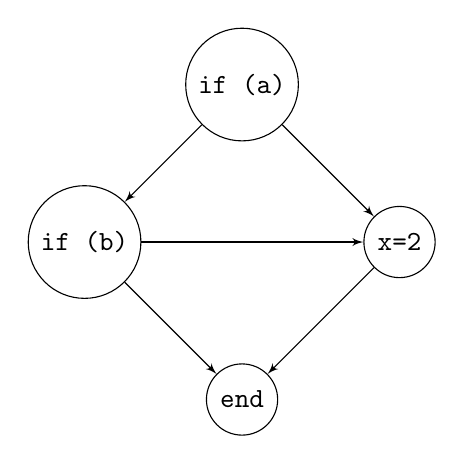
\begin{tikzpicture}
        \tikzset{vertex/.style = {shape=circle,draw,minimum size=2.5em}};
        \tikzset{edge/.style = {->,> = latex'}};
        \node[vertex] (a) at (2,8) {\texttt{if (a)}};
        \node[vertex] (b) at (0,6) {\texttt{if (b)}};
        \node[vertex] (c) at (4,6) {\texttt{x=2}};
        \node[vertex] (d) at (2,4) {\texttt{end}};
        \draw[edge] (a)  to (b);
        \draw[edge] (a)  to (c);
        \draw[edge] (b)  to (c);
        \draw[edge] (b)  to (d);
        \draw[edge] (c)  to (d);
    \end{tikzpicture}
    \caption{Cyclomatic complexity graph for Figure~\ref{c1excode}}
    \label{fig:c1exgraph}
\end{figure}

\subsection{Cyclomatic Complexity in Functional
Programming}

The definition of cyclomatic complexity in Section~\ref{cyclomaticcomplexity} is
not ideal for functional programming. Cyclomatic complexity is calculated by
creating graphs based on control flow operations such as while loops and if
statements. In functional programming everything is a function, thus the
cyclomatic complexity will always tend to 0 using this definition. So we define
a different method of calculating the cyclomatic complexity for functional
programs. 

\theoremstyle{definition} 
    \begin{definition} 
    The cyclomatic complexity number, in functional programming, is equal to
    1 plus the sum of the left hand side, called LHS, plus the sum of the
    right hand side, called RHS. RHS is the sum of the number of guards,
    logical operators, filters in a list comprehension and the pattern
    complexity in a list comprehension. LHS is equal to the pattern
    complexity.  The pattern complexity is equal to the number of
    identifiers in the pattern, minus the number of unique identifiers in
    the pattern plus the number of arguments that are not identifiers. In
    summary:

    \begin{lstlisting}
    Cyclomatic complexity = 1 + LHS + RHS

    LHS = Pattern complexity 

    Pattern complexity   
        = Pattern identifiers 
        - Unique pattern identifiers 
        + Number of arguments that are non identifiers

    RHS = Number of guards 
        + Number of Logical operators 
        + Number of filters in list comprehension 
        + Pattern complexity in list comprehension
    \end{lstlisting}
\end{definition}

Instead of cyclomatic graphs in functional programs one constructs flowgraphs,
such as the one seen in Figure~\ref{fig:cyclomaticfunctional}, to model the
functions.

\begin{figure}[H]
    \begin{lstlisting}
    split :: (a -> Bool) -> [a] -> ([a], [a])
    split onCondition [] = ([], [])
    split onCondition (x:xs) =
        let 
            (ys, zs) = split onCondition xs
        in 
            if (onCondition x) then 
                (x:ys, zs)
            else 
                (ys, x:zs)
    \end{lstlisting}
    \caption{Recursively split a list into two based on a given condition in
    Haskell. For example \texttt{split (>3) [1,2,3,4,5] =
    ([4,5],[1,2,3])}.}
    \label{split}
\end{figure}

In Haskell $(x:xs)$ denotes an item $x$ at head of a list of items $xs$. Given
the Haskell code in Figure~\ref{split}. To calculate LHS we find two
pattern identifiers which are $onCondition$ and $(x:xs)$. there is one unique
pattern identifiers which is $(x:xs)$. There is also one non identifier
which is $[]$. There is also one guard, an if statement, and no
list comprehensions on RHS. Thus the cyclomatic complexity is $1+(2-1+1)+1=4$.

In this method to calculate cyclomatic complexity, do not count the $otherwise$
and $else$ clauses.~\cite{bergklaas}


\begin{figure}[H]
    \centering
    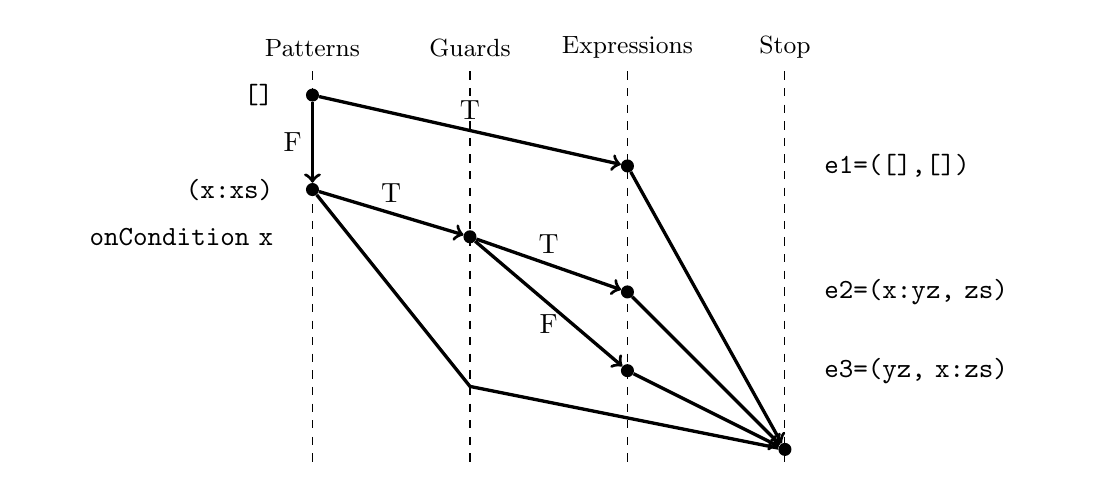
\begin{tikzpicture}
        \tikzset{vertex/.style = {shape=circle,fill=black,scale=0.5}};
        \draw[dashed] (0,0) -- (0,-5) (2,0) -- (2,-5) (4, 0) -- (4, -5) (6, 0)
        -- (6, -5);
        \node at (0,.3) {\small{Patterns}};
        \node at (2,.3) {\small{Guards}};
        \node at (4,.3) {\small{Expressions}};
        \node at (6,.3) {\small{Stop}};
        \node[vertex] (a) at (0,-0.3) {};
        \node[align=right, text width=3cm] at (-2,-0.3) {\texttt{[]}};
        \node[vertex] (b) at (4,-1.2) {};
        \draw[->, very thick] (a) to node [above] (TextNode) {T} (b) ;
        \node[vertex] (c) at (0,-1.5) {};
        \node[align=right, text width=3cm] at (-2,-1.5) {\texttt{(x:xs)}};
        \draw[->, very thick] (a) to node [left] (TextNode) {F} (c) ;
        \node[align=left, text width=3cm] at (8,-1.2) {\texttt{e1=([],[])}};
        \node[vertex] (d) at (2,-2.1) {};
        \draw[->, very thick] (c) to node [above] (TextNode) {T} (d) ;
        \node[align=right, text width=3cm] at (-2,-2.1) {\texttt{onCondition x}};
        \node[vertex] (e) at (4,-2.8) {};
        \draw[->, very thick] (d) to node [above] (TextNode) {T} (e) ;
        \node[align=left, text width=3cm] at (8,-2.8) {\texttt{e2=(x:yz, zs)}};
        \node[vertex] (f) at (4,-3.8) {};
        \draw[->, very thick] (d) to node [below] (TextNode) {F} (f) ;
        \node[align=left, text width=3cm] at (8,-3.8) {\texttt{e3=(yz, x:zs)}};
        \node[vertex] (g) at (6,-4.8) {};
        \draw[->, very thick] (e) to (g) ;
        \draw[->, very thick] (b) to (g) ;
        \draw[->, very thick] (f) to (g) ;
        \draw[very thick] (c) to (2, -4.0) to (g) ;
    \end{tikzpicture}
    \caption{Flowgraph for split function, defined in Figure~\ref{split}.}
    \label{fig:cyclomaticfunctional}
\end{figure}

Cyclomatic complexity finds how many tests are needed to get full branch
coverage of source code. A low complexity for a program means that less tests
have to be written.  Note that if a program has a low cyclomatic complexity it
does not imply that the program is easier to test. If a program is written in
such a way that it depends heavily on the environment it can also lead to
difficulty testing. So to make cyclomatic complexity a better metric this study
will use design patterns to make testable code.

\subsection{Mental complexity: Cognitive Dimensions}\label{cognitivedimensions}

Cognitive Dimensions is a framework for evaluating the usability of programming
languages and to find areas of improvements.~\cite{GREEN1996131} It allows us to
evaluate the quality of a design and explore what future improvements could be
made. As part of the Cognitive Dimensions, 14 different Cognitive Dimensions of
Notation exist. A notation depends on the specific context, in this case the
notation is the languages themselves and their architecture. The author of the
framework recommends omitting the dimensions that are not applicable to the
notation. We give a brief description of the dimensions.

\begin{description}

\item[ Viscosity ]

How much work does it take to make small changes? How easy is the code to
refactor? If small changes requires consequent adjustments then that is a
problem. As a viscous system cause a lot more work for the user and break the
line of thought.

\item[ Visibility ]

How easy is it to navigate the source code to find the parts that you want?

\item[ Hidden dependencies ]

Are there hidden dependencies in the source code. Does a change in one part of
the source code lead to unexpected consequences in another part of the code.
Every dependency that matters to the user should be accessible in both
directions. 

\item[ Role-expressiveness ]

How obvious is each sub-component of the source code to the solution as a whole?

\item[ Abstraction ]

What are the levels of abstraction in the source code? Can the details be
encapsulated?

\item[ Secondary notation ]

Are there any extra information being conveyed to the user in the source code?

\item[ Closeness of mapping ]

By looking at the source code, how close do we find it to be to the case
we are solving?

\item[ Consistency ]

Once Object-oriented procedural programming and Functional programming has been
learned. How much of the rest can the user guess successfully? 

\item[ Diffuseness or terseness ]

How much space and symbols does the source code need to produce a certain result
or express a meaning?

\item[ Hard mental operations ]

Where does the hard mental processing lie? Is it more when writing the source
code itself rather than solving the case, I.E. the semantic level? Does one
sometimes need to resort to pen and paper to keep track of what is happening?

\item[ Provisionality ]

How easy is it to get feedback of something before you have completed the entire
system?

\item[ Progressive evaluation ]

How obvious the role of each component of the source code in the solution as a
whole?

\item[ Error proneness ]

To what extent does the programming paradigm and language help minimise errors? Are
there any structures or complexities that lead to it being easier to make
errors?
\end{description}

\noindent For this study we will investigate the following dimensions: 

\begin{itemize}
    \item Diffuseness or terseness
    \item Progressive evaluation
    \item Closeness of mapping
    \item Hard Mental Operations
    \item Visibility
    \item Hidden dependencies
    \item Abstraction
    \item Error-proneness 
\end{itemize}

\noindent We omit the other dimensions as related work concluded that the other
dimensions did not bring much weight when evaluating the different
paradigms.~\cite{euguenkiss}

In summary, cognitive dimensions allow us to look at different aspects of a
programming language to evaluate how complex they are cognitively. 



% Theory 
\chapter{Method}

To evalute if the functional approach to creating servers is more maintainable
than existing solutions, a comparative study will be done. A popular library for
developing server applications is by using an unopiniated solution using
Express, which is a good candidate to compare to Cause.

Express is an unopiniated server framework written for Node.js for Javascript.
That a framework is unopiniated means that it does not force you to architecture
your code in any specific way.  

\section{Constructing the server in Express and Cause}

To measure the maintainability, a comparison will be made by comparing a correct
construction of an idiomatic server both made in Cause and the popular framework
for Node Express. They will feature similar functionality which is a library api
with the endpoints:

\begin{itemize}
    \item \texttt{GET ``api/books?released=int\&author=string''} Get a list of
    books and optionally ask for a specific author or a book from a specific
    year
    \item \texttt{DELETE ``api/books/:id''} Delete a book with a specified ID.
    \item \texttt{POST ``api/books/:id'' OR ``api/books/''} Create a new book or
    override a specific book
\end{itemize}

The server will also make use of a hashmap for database connection.

The accepted content types will be \texttt{application/json} and
\texttt{www-url-formencoded} for all endpoints and the displayable content-types
are \texttt{text/plain} and \texttt{application/json}. Both implementations will handle
all of the error cases. They will also be written in an idiomatic way, that is
they will not take the challenges outlined in Chapter~\ref{background} into
consideration; the only requirement is that they compile.

\section{Evaluating maintainability}

The aspects that to be evaluated when measuring maintainability were discussed
in Chapter~\ref{background}. This study will focus on evaluating the following
criterias:

\begin{itemize}
    \item Testability
    \item Extendability
    \item Readability
    \item Error-proneness
\end{itemize}

Each of them require a different approach for evaluation.

\subsection{Evaluating testability}

The testability of the code is determined by it's aherence to SOLID principles,
in particular of it's use of inversion of control. If a solution has less
dependencies, it becomes easier to use unit tests to test the code and less
resources are needed to create integration tests and E2E-tests.

Evaluation can be done then by counting the amount of mocked dependencies in the
imperative solution and the functional solution.

\subsection{Evaluating error-proneness and extendability}

To evaluate error-proneness and extendability an expert analysis will be used.
Cognitive Dimensions is a framework for evaluating the usability of programming
languages and to find areas of improvements.~\cite{GREEN1996131} It allows us to
evaluate the quality of a design and explore what future improvements could be
made. As part of the Cognitive Dimensions, 14 different Cognitive Dimensions of
Notation exist. A notation depends on the specific context, in this case the
notation is the languages themselves and their architecture. The author of the
framework recommends omitting the dimensions that are not applicable to the
notation. This framework is used to evaluate the safety, error-proneness and
extendability of both the Express and Cause solution.

\begin{description}

\item[ Viscosity ]

How much work does it take to make small changes? How easy is the code to
refactor? If small changes requires consequent adjustments then that is a
problem. As a viscous system cause a lot more work for the user and break the
line of thought.

\item[ Visibility ]

How easy is it to navigate the source code to find the parts that you want?

\item[ Hidden dependencies ]

Are there hidden dependencies in the source code. Does a change in one part of
the source code lead to unexpected consequences in another part of the code.
Every dependency that matters to the user should be accessible in both
directions. 

\item[ Role-expressiveness ]

How obvious is each sub-component of the source code to the solution as a whole?

\item[ Abstraction ]

What are the levels of abstraction in the source code? Can the details be
encapsulated?

\item[ Secondary notation ]

Are there any extra information being conveyed to the user in the source code?

\item[ Closeness of mapping ]

By looking at the source code, how close do we find it to be to the case
we are solving?

\item[ Consistency ]

How much of the rest can the user guess 

\item[ Diffuseness or terseness ]

How much space and symbols does the source code need to produce a certain result
or express a meaning?

\item[ Hard mental operations ]

Where does the hard mental processing lie? Is it more when writing the source
code itself rather than solving the case, I.E. the semantic level? Does one
sometimes need to resort to pen and paper to keep track of what is happening?

\item[ Provisionality ]

How easy is it to get feedback of something before you have completed the entire
system?

\item[ Progressive evaluation ]

How obvious the role of each component of the source code in the solution as a
whole?

\item[ Error proneness ]

To what extent does the programming paradigm and language help minimise errors? Are
there any structures or complexities that lead to it being easier to make
errors?
\end{description}

\noindent For this study we will investigate the following dimensions: 

\begin{itemize}
    \item Diffuseness or terseness
    \item Closeness of mapping
    \item Hard Mental Operations
    \item Visibility
    \item Hidden dependencies
    \item Abstraction
    \item Error-proneness 
\end{itemize}

\noindent We omit the other dimensions as related work concluded that the other
dimensions did not bring much weight when evaluating the different
paradigms.~\cite{euguenkiss}

These aspects can also give us insights in the other aspects of mainatainability
and will be used for discussion and evaluation.

\subsection{Evaluating readability through code reviews}

Code reviews, also known as peer reviews, is an activity where a human evaluates
the program to check for defects, finding better solutions and find readability
aspects. 

To measure the readability of the REST library, a semi-structured code review is
conducted on five different people with varying knowledge of REST apis and
functional programming.

\subsubsection{Semi-structured interviews}

Semi-structured interviews diverges from a structured interview which has a set
amount of questions. In a semi-structured interview the interview is open and
allows for new ideas to enter the discussion. 

Semi-structured interviews are used to gather focused qualitative data. It is
useful for finding specific insights in regards to the readability of the code
and provides insights as to wether or not the code can actually be understood by
the general user.

To conduct an semi-structured interview, the interview should avoid leading
questions and use open-ended questions to get descriptive answers rather than
yes or no answers. 

The questions that will be asked are presented below.

\begin{itemize}
    \item What is your experience with Express?
    \item What is your experience with ReasonML?
    \item After being presented the code api, can you explain what it does?
    \item Which media types does the endpoint accept?
    \item Which media types representations can the endpoint show?
    \item Can you demonstrate how you would extend the api and add a new endpoint
    for a PUT request.
\end{itemize}

\subsection{Evaluating the answers}

After performing the interviews conclusions can be made by having the author
interprate the answers to conclude if the code is readable or not. If the code
is readable the users being interviewed should be able to explain to the author
what the code does.

In order to reduce the bias in the experiments each user will be shown a
different code base first. So the 3 users will be shown the implementation in
ReasonML and 2 users will be shown the implementation in Express.

So in summary, the way each aspect of maintainability will be evaluated in both
solutions by the following:

\begin{description}
    \item [Testability] Evaulated by comparing the number of dependencies that
    need to be mocked. 
    \item [Extendability] Evaluated by analysing the results from cognitive
    dimensions and the interviews.
    \item [Readability] Evaluated by merging the results of cognitive dimensions
    and the interviews.
    \item [Error-proneness] Evaluated by analysing the results from cognitive
    dimensions and the interviews.
\end{description}

Afterwards from there a discussion can be had about the strenghts and weaknesses
of both solutions and the impacts of maintainability by using functional
programming for developing REST servers.






\chapter{Results}\label{results}
We worked so hard, yet achieved very little. TODO

\section{Limitations}\label{limitations}

TODO

\subsection{Improvements to implementation}
TODO

\section{future work}
\subsection{Relations to cardinality}
TODO

\bibliographystyle{ieeetr}
\bibliography{thesis}

\end{document}
